\newpage
\begin{center}
\textbf{\large ГЛАВА 1 \\ Роль дальнодействия притяжения в коллективной динамике простых жидкостей}
\end{center}
\refstepcounter{chapter}


\addcontentsline{toc}{chapter}{ГЛАВА 1. Роль дальнодействия притяжения в простых жидкостях}

\section{Влияние дальнодействия потенциала на критическое поведение}

Многие из межмолекулярных сил, играющих центральную роль в обширных областях химии, физики и биологии, имеют дальнодействующую природу.
Хорошо известными примерами являются электростатические взаимодействия, силы поляризации и силы Ван-дер-Ваальса.
Примечательно, что в наших знаниях о критическом поведении, вызванном этими взаимодействиями, все еще имеются значительные недостатки.

Нынешнее понимание критического поведения в системах с такими алгебраически затухающими взаимодействиями в значительной степени основано на расчетах ренормализационной группы.
Показано, что для универсальных критических свойств можно выделить разные режимы, характеризуемые затухающей мощностью взаимодействий.
Ввиду небольшого числа глобальных параметров, определяющих класс универсальности, значительный интерес представляет расположение границ между этими режимами.

В данном разделе рассматриваются границы между режимами взаимодействия, которые определяют класс универсальности. 

Данный подход специализируется на модели Изинга, $n = 1$, в $d$ измерениях, описываемой редуцированным гамильтонианом
\begin{equation}
\mathcal{H} / k_{\mathrm{B}} T=-K \sum_{\langle i j\rangle} \frac{s_{i} s_{j}}{r_{i j}^{d+\sigma}}
\label{eq1}
\end{equation}

где спины $s_{k}=\pm 1$ помечены узлом решетки $k$, сумма распространяется на все пары спинов, а связь пар зависит от расстояния $r_{i j}=\left|\vec {r}_{i}-\vec{r}_{j}\right|$ между спинами. Согласно анализу Фишера~\cite{10.1103/PhysRevLett.29.917} классы универсальности параметризованы $\sigma$, и были определены следующие три различных режима: (a) классический режим; верхняя критическая размерность определяется как $d_{u}=2\sigma$, так что критическое поведение типа среднего поля возникает при $\sigma \leq d / 2$. (б) промежуточный режим $d/2<\sigma<2$; здесь критические показатели являются непрерывными функциями от $\sigma$. (c) режим ближнего действия; для $\sigma\geq 2$ универсальными являются свойства модели с короткодействующими взаимодействиями, например, только между ближайшими соседями; таким образом, можно заметить, что при $d=3$ ван-дер-ваальсовы взаимодействия (затухающие как $1/r^{6}$) действительно лежат довольно близко к границе между режимами (b) и (c).

Хотя общий план этих результатов получил широкое признание, одна часть этой картины стала предметом споров. Это касается ситуации, близкой к $\sigma=2$. В работе~\cite{10.1103/PhysRevLett.29.917} было высказано предположение, что во всем промежуточном режиме (b) показатель корреляционной функции $\eta$ в точности равен $2-\sigma$. С другой стороны, в короткодействующем режиме (в) $\eta$ принимает постоянное (но зависящее от $d$) значение $\eta_{\mathrm{sr}}>0$ для всех $d<4 $, что приводит к скачку разрыва в $\eta$ при степени затухания $\sigma=2$. Хотя это замечательное явление не запрещается термодинамическими аргументами (для которых требуется только $\eta\leq 2+\sigma$ ), оно привлекло значительное внимание в последние десятилетия, и были предприняты различные усилия для повторного исследования соответствующего сценария $R G$~\cite{10.1103/PhysRevB.8.281, 10.1088/0305-4470/22/6/024}. Кроме того, можно отметить, что этот сценарий не охватывает одномерный случай, когда строго известно~\cite{10.1007/BF01654281} отсутствие фазового перехода при $\sigma>1$, а не при $\sigma>2$. Первым к этому вопросу обратился Сак~\cite{10.1103/PhysRevB.8.281}, который указал, что члены высших порядков в уравнениях $RG$, рассмотренных в~\cite{10.1103/PhysRevLett.29.917} генерируют дополнительные короткодействующие взаимодействия в процессе перенормировки, что влияет на конкуренцию между дальнодействующими и короткодействующими неподвижными точками $RG$-преобразования.

Как следствие, при $d<4$ граница между промежуточным и ближним режимами смещается от $\sigma=2$ к $\sigma=2-\tilde{\eta}$, где Разложение $\varepsilon$ для $\tilde{\eta}$ согласуется в низших порядках с разложением ближнего показателя $\eta_{\mathrm{sr}}$. 
Используя теоретико-полевой подход, Хонконен и Налимов~\cite{10.1088/0305-4470/22/6/024} доказали во всех порядках теории возмущений устойчивость малодействующей неподвижной точки при $\sigma>2-\eta_{\mathrm{sr}}$ и его дальнодействующий аналог для $\sigma<2-\eta_{\mathrm{lr}}$, где $\eta_{\text {lr }}$ — аномальная размерность поля, оцененная при фиксированном дальнодействии. Обратите внимание, что эти авторы также указали, что первый результат может быть получен из простых аргументов масштабирования, а второй - нет. Привлекательными аспектами этих результатов являются, во-первых, непрерывная и монотонная $\sigma$-зависимость показателя корреляционной функции (при условии, что $\eta_{\mathrm{Ir}}$ и $\eta_{\mathrm{sr}}$ совпадают при $\sigma=2-\eta_{\mathrm{sr}}$ ), и, во-вторых, что теперь теория достигла согласованности с точными результатами для одномерного случая.

Поскольку основная проблема в моделировании заключается в переходной области между промежуточным режимом и режимом ближнего действия, можно ожидать, что поправки к масштабированию будут сходиться медленно с увеличением размера системы. Это требует моделирования больших систем. Использование кластерного алгоритма Монте-Карло~\cite{10.1142/S0129183195000265}, использующего число операций на переворот спина, не зависящее от размера системы, и, кроме того, подавляющее критическое замедление, в настоящее время позволило получить высокоточные данные для достаточно больших размеров системы.

Для представления численных результатов критического показателя вычисляется $\eta$ и кумулянт Биндера~\cite{10.1007/BF01293604} в зависимости от $\sigma$. Моделируемые системы задаются на решетках $L\times L$ с периодическими границами и размерами от $L=4$ до $L=1000$. 
Для изучения выбираются двумерные системы не только для максимизации достижимого линейного размера системы, но, в частности, потому, что показатель степени $\eta_{\mathrm{sr}}=\frac{1}{4}$ имеет гораздо большее значение, чем при $d=3\left(\eta_{\mathrm{sr}}=0.037\right)$. Это максимизирует как размер спорной области $\left\langle 2-\eta_{\mathrm{sr}}, 2\right\rangle$, так и величину предполагаемого скачка $\eta(\sigma)$. Продолжительность моделирования выбирается такой, что (для систем самых больших размеров) достигается относительная неопределенность в одну тысячную для кумулянта Биндера. Точная форма парного взаимодействия принимается как:

\begin{equation}
\tilde{K}(|\vec{r}|)=K \int_{r_{x}-(1 / 2)}^{r_{x}+(1 / 2)} d x \int_{r_{y}-(1 / 2)}^{r_{y}+(1 / 2)} d y \frac{1}{\left(x^{2}+y^{2}\right)^{(d+\sigma) / 2}}
\end{equation}

где $\vec r=\left(r_{x}, r_{y}\right)$ обозначает разность между целыми координатами двух взаимодействующих спинов. Важно отметить, что это взаимодействие, принятое из чисто технических соображений~\cite{10.1142/S0129183195000265}, отличается от взаимодействия в уравнении\ref{eq1} только в степенях $r$, убывающих быстрее, чем $r^{-d-\sigma}$. Критические индексы и границы режимов (а)–(c) не изменятся. 

Важной проблемой в этих анализах является тот факт, что показатели степени коррекции к масштабированию по существу неизвестны и фактически зависят от граничного значения $\sigma$. Предприняты значительные усилия, чтобы охватить все такие неопределенности в указанных полях для оценки $K_{c}$, $Q$, $\eta$.

Таким образом, как показатель корреляционной функции $\eta$, так и отношение амплитуд четвертого порядка $Q$ принимают свои (универсальные) короткодействующие изинговские значения для $\sigma>2-\eta_{\mathrm{sr}}$. Для $\sigma>2$ это можно показать с высокой численной точностью, а для $2-\eta_{\mathrm{sr}}<\sigma<2$ результаты достаточно точны, чтобы убедительно исключить переход от дальнодействующего критического поведения к ближнедействующему при $\sigma=2$ . Вместо этого они поддерживают кроссовер при $\sigma=2-\eta_{\mathrm{sr}}$. 
Эти результаты прекрасно согласуются с $\eta=2-\sigma$ в промежуточном диапазоне $d/2<\sigma<2-\eta_{\mathrm{sr}}$, подтверждая гипотезу о том, что все вклады высших порядков обращаются в нуль в разложении $\varepsilon^{\prime}$ для $\sigma$ ~\cite{10.1103/PhysRevLett.29.917}. Отношение амплитуд $Q$ зависит примерно линейно на $\sigma$ для $d/2<\sigma<2-\eta_{\mathrm{sr}}$. 
Примечательно, что наиболее заметные отклонения от линейности возникают вблизи $\sigma=2-\eta_{\mathrm{sr}}$, в то время как разложение $\varepsilon^{\prime}$ предсказывает сингулярность, подобную квадратному корню, на противоположном конце промежуточного диапазона ~ \cite{10.1103/PhysRevE.60.7558}.


\section{Влияние дальнодействия потенциала на фазовые диаграммы и плавление}

Понимание фазовых переходов в 2D-системах имеет большое значение в ряде областей, от фотоники и электроники до новых материалов и биотехнологий, поскольку знание фазового поведения открывает путь к проектированию систем с желаемыми свойствами. Несмотря на многочисленные исследования, основные вопросы здесь по-прежнему связаны с влиянием конкретного взаимодействия между отдельными частицами на их коллективное поведение. Для классических систем одной из простейших моделей, способных воспроизвести их поведение, включая газовую, жидкую и твердую фазы, является система Леннарда-Джонса (LJ). Модель LJ широко используется для анализа поведения молекулярных, белковых, полимерных, эмульсионных и коллоидных мягких веществ. Обобщенный LJ-потенциал (или LJn-m-потенциал, где индексы n и m отвечают за алгебраические ветви отталкивания и притяжения) является подходящей моделью для исследований, направленных на выявление эффектов отталкивания и притяжения на жидкости, твердые тела и фазовый переход между ними.

В настоящий момент установлено, что 2D-сценарии плавления зависят от мягкости отталкивания, обеспечивая следующие микроскопические сценарии 2D-плавления~\cite{10.3367/ufne.2017.06.038161, 10.3367/ufne.2018.04.038417}: теория Березинского-Костерлица-Таулесса-Гальперина-Нельсона-Юнга (БКТГНЮ), согласно которой плавление происходит через два непрерывных перехода с промежуточной гексатической фазой с квазидальним ориентационным порядком и ближним трансляционным порядком~\cite{10.1088/0022-3719/6/7/010, 10.1103/physrevlett.41.121, 10.1103/physrevb.19.2457, 10.1103/physrevb.19.1855}, плавление через фазовый переход первого рода; двухстадийное плавление, включающее непрерывный (Березинский-Костерлиц-Таулесс, БКТ) кристаллогексатический фазовый переход и фазовый переход первого рода между гексатической фазой и изотропной жидкостью.
Второй и третий сценарии присущи твердым сфероподобным системам, тогда как первый наблюдался при мягком отталкивании между частицами. Однозначно установлено, что мягкость отталкивания влияет на сценарии плавления, термодинамику и спектры возбуждения в монослойных системах. Однако, насколько нам известно, роль притяжения в сценарии плавления монослойных систем остается систематически неизученной.

LJ-взаимодействия были одними из первых систем, изученных для понимания роли притяжения в плавлении. Тем не менее, многие опубликованные результаты по критической точке и сценарию плавления для 2D-кристаллов LJ все еще остаются сомнительными. Например, чтобы обеспечить критическую температуру в зависимости от радиуса усечения, было выполнено численное моделирование кривой пар-жидкость в ансамбле Гиббса, как сообщалось в~\cite{10.1063/1.460477}. Для критической температуры и плотности авторы получили $T_c =0,515 \pm 0,002$ и $\rho_c = 0,355 \pm 0,003$ соответственно для полного потенциала; и $T_c = 0,459\pm 0,001$ и $\rho_c = 0,35\pm 0,01$ для усеченного и сдвинутого потенциала при $2,5\sigma$. 
О противоречивых сценариях плавления треугольного кристалла сообщалось в ранних работах~\cite{10.1103/physrevlett.42.1632, 10.1063/1.436526, 10.1103/physrevlett.44.463, 10.1063/1.441901, 10.1103/physrevlett.52.449, 10.1103/physrevb.30.2755}, включая два непрерывных перехода с промежуточной гексатической фазой по теории БКТГНЮ~\cite{10.1103/physrevlett.42.1632} и переход первого рода ~\cite{10.1063/1.436526, 10.1103/physrevlett.44.463, 10.1063/1.441901, 10.1103/physrevlett.52.449}.

Благодаря росту вычислительных возможностей моделирование больших систем ($\gtrsim 10^5$ частиц) недавно дало новые результаты по двумерному плавлению кристаллов Леннарда-Джонса и связанных с ними систем. Моделирование систем с последующим анализом их уравнения состояния и дальнодействующей асимптотики трансляционной корреляционной функции (которая точно обеспечивает предел устойчивости кристалла) позволило однозначно идентифицировать сценарии плавления. Например, об изменении сценария плавления сообщалось в работе~\cite{10.1103/physreve.99.022145}, где авторы изучали двумерные системы частиц, взаимодействующих посредством обобщенного потенциала Леннарда-Джонса с различными ветвями отталкивания ($\propto 1/r ^{12}$ и $\propto 1/r^{64}$). Установлено, что сценарий реализуется через фазовые переходы первого рода при низких температурах и через два непрерывных перехода БКТ (согласно теории БКТГНЮ) при высоких. Обычно предполагается, что LJ-система при высоких температурах близка к мягким отталкивающим дискам $1/r^{12}$, но такая экстраполяция на сценарий плавления противоречит результатам работы~\cite{10.1103/physrevlett.114.035702}, где показано, что мягкие диски $1/r^n$ с $n>6$ плавятся по третьему сценарию плавления. Предполагается, что петля Майера-Вуда, присущая переходу первого рода, исчезает при высоких температурах с увеличением размера системы. Однако объяснение эффекта конечно-размерным масштабированием кажется неубедительным: с увеличением размера системы петля должна сплющиваться и в конечном итоге приближаться к плато ~\cite{10.1103/physreve.87.042134, 10.1103/physreve.59.2659}.

Было установлено, что при низких температурах, где преобладает роль притяжения, все системы плавятся по переходу первого рода за счет подавления гексатической фазы. При высоких температурах LJ-диски плавятся по третьему сценарию, как и мягкие диски ~\cite{10.1103/physrevlett.114.035702}, тогда как шестиугольники и квадраты по теории БКТГНЮ. Сценарий плавления пентагонов не меняется с повышением температуры и является переходом первого рода.

Показано, что кристаллы LJ по сравнению с системой Морзе в~\cite{10.1103/physrevb.103.094107} плавятся по третьему сценарию при низких температурах и два непрерывных перехода БКТ при высоких. Это согласуется с~\cite{10.1103/physreve.99.022145}, но противоречит~\cite{10.1103/physrevlett.114.035702}. Сценарий БКТГНЮ при высоких температурах был поставлен под сомнение из-за кажущегося исчезновения петли Майера-Вуда (аналога петли Ван-дер-Ваальса в трехмерном случае). Для мягких взаимодействий Морзе третий сценарий плавления наблюдается для всех температур, рассмотренных в~\cite{10.1103/physrevb.103.094107}, тогда как авторы ожидали наблюдать сценарий БКТГНЮ при более высоких температурах. Однако при некоторых параметрах потенциальной мягкости уже при низких температурах при наличии дальнодействующего притяжения наблюдались два непрерывных перехода.

Роль притяжения можно проверить экспериментально в коллоидных системах, давно известных как модельные системы, демонстрирующие широкий спектр ``молекулярно-подобных'' явлений~\cite{book.fernandez, book.ivlev, 10.1016/0370-1573(94)90017-5, 10.1038/natrevmats.2015.11, 10.1039/c9sm01953g}, в частности кристаллизация и плавление~\cite{10.1126/science.1112399, 10.1039/c2sm26473k, 10.1103/physrevlett.82.2721, 10.1103/physrevlett.85.3656, 10.1103/physrevlett.118.088003, 10.1039/c2sm27654b, 10.1126/science.1224763, 10.1038/s41598-021-97124-7}.

Эти коллективные явления можно визуализировать в реальном времени с пространственным разрешением отдельных частиц. Дальнодействующее диполярное притяжение $\propto 1/r^3$ в коллоидных системах можно индуцировать и контролировать in situ с помощью вращающегося в плоскости магнитного поля~\cite{10.1088/0034-4885/76/12/126601, 10.1039/c3sm50306b, 10.1039/c3sm27620a, 10.1103/physrevmaterials.2.025602} или электрического~\cite{10.1088/1367-2630/8/11/267, 10.1063/1.3115641, 10.1021/la2014804, 10.1021/la500178b, 10.1039/c1sm06414b, 10.1038/s41598-017-14001-y} поля.
Используя конически вращающиеся магнитные или электрические поля с магическими углами, можно создать ван-дер-ваальсово притяжение $\propto 1/r^6$ с "магическими" полями \cite{10.1021/la500896e, 10.1103/physrevlett.103.228301}.
В последнее время настраиваемые взаимодействия были достигнуты за счет использования пространственных годографов внешнего электрического или магнитного поля~\cite{10.1039/d0sm01046d}, проектирования внутренней структуры~\cite{10.1063/5.0055566} и геометрии~\cite{10.1063/5.0060705} коллоидных частиц.

Исследование систем частиц производится посредством обобщенного потенциала Леннарда-Джонса (LJn-m):

\begin{equation}
U_{n m}(r)=\frac{\epsilon}{n-m}\left[m\left(\frac{\sigma}{r}\right)^{n}-n\left(\frac{\sigma}{r}\right)^{m}\right]
\end{equation}

где $n$ и $m$ — индексы отталкивающей и притягивающей ветвей соответственно, а $\sigma$ и $\epsilon$ — характерная длина взаимодействия и глубина потенциальной ямы. Потенциал имеет минимум $-\epsilon$ при $r/\sigma=1$. В дальнейшем нормируются расстояния и энергии на $\sigma$ и $\epsilon$ соответственно и рассматриваются частицы одинаковой массы $m=1$.

Результаты для бинодального конденсата-газа, полученные с помощью метода фазовой идентификации и уравнения состояния, представлены на рисунке~\ref{nmp}. Здесь цветными кружками обозначены плотности газа, конденсата и их среднее значение для каждого рассмотренного нами потенциала. Сплошными серыми линиями показаны области данных, в которых использовали аппроксимацию для получения данных о критической точке. Серыми пунктирными линиями показана экстраполяция фазовой диаграммы на критические точки газ-жидкость, обозначенные цветными звездочками.

\begin{figure}[!h]
\begin{center}
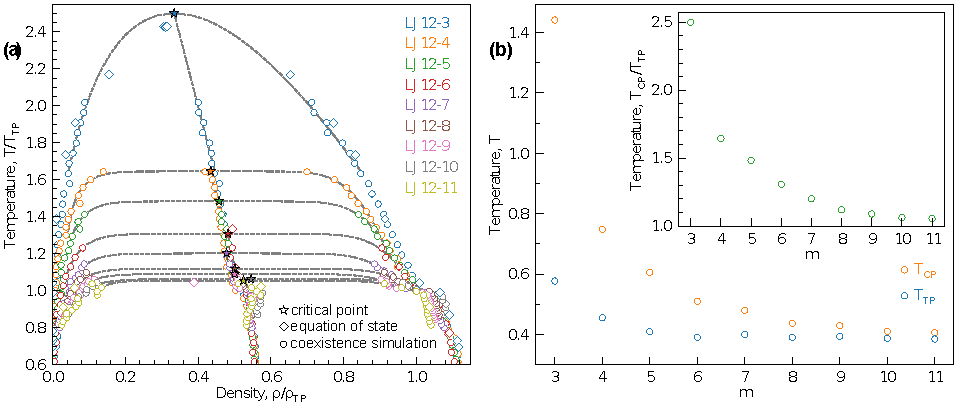
\includegraphics[width=\textwidth]{NMP-Figure4.pdf}
\caption{Влияние диапазона притяжения на область сосуществования жидкость-газ на фазовой диаграмме: (a) бинодали конденсат-газ для разных потенциалов LJ12-m; кружки — точки бинодали и медианы (полученные методом фазовой идентификации), ромбы — точки, полученные из уравнения состояния, серые линии — аппроксимации бинодали, звездочками обозначены критические точки. (b) Зависимости тройной и критической температур от индекса притяжения m для взаимодействия LJ12-m, отношение $T_{CP}$/$T_{TP}$ показано на вставке.}
\label{nmp}
\end{center}
\end{figure}

Падение диапазона притяжения снижает критическую температуру, а также отношение между температурами критической и тройной точек, как показано на рисунке~\ref{nmp}(b) и соответствующей вставке. С увеличением $m$ (ближнее притяжение) двухфазная область сужается в сторону меньших плотностей, а отношение между критической и тройной температурами становится ближе к единице. Для LJ-взаимодействия ($m = 6$) полученная критическая температура $Tc = (0,51 . . . 0,52)$ (в зависимости от метода оценки) хорошо согласуется с предыдущими результатами $T_c = 0.515 \pm 0.002$  для LJ-потенциала.

В данном разделе был проведен обзор эволюции фазовых диаграмм и сценариев плавления двумерных систем частиц, взаимодействующих через обобщенный потенциал Леннарда-Джонса с разным диапазоном притяжения, тогда как ветвь отталкивания была зафиксирована. Газожидкостный переход изучается с помощью анализа уравнения состояния и метода фазовой идентификации. Результаты, полученные двумя методами, хорошо согласуются, что свидетельствует об их согласованности. Плавление при высоких температурах (и высоких плотностях) ведет себя как система мягких дисков $1/r_{12}$ по третьему сценарию. Однако при низких температурах плавления идет смена сценария плавления от третьего сценария к переходу первого рода (без гексатической фазы) в системах с $m = 6$, $9$ и $11$. Температура изменения сценариев смещаются в сторону более низких температур с увеличением диапазона притяжения (соответствующего уменьшению $m$). Анализ случая $m = 9 (LJ12-9)$  показал, что для короткодействующего притяжения в сложных растворителях можно наблюдать третий сценарий плавления.

Однако на данный момент не существует теории, которая предсказывала бы поведение транспортных свойств и коллективных возбуждений в зависимости от дальнодействия притяжения. В связи с этим формулируются следующие цели и задачи настоящей работы.

\section{Цели и задачи магистерской работы}

\textbf{Цель работы} -- установить связь дальнодействия притяжения потенциала и спектров возбуждений с транспортными свойствами жидкостей, а также влияние на скорость нуклеации.

\textbf{Задачи работы:}
\begin{enumerate}
    \item Расчет фазовых диаграмм для 2D и 3D систем частиц, взаимодействующих посредством обобщенного потенциала Леннарда--Джонса с различными степенями притяжения.
    \item Адаптация метода кластеризации данных DBSCAN для изучения молекулярных систем и его сравнение с другими методами.
    \item Расчет и анализ транспортных свойств и коллективных возбуждений на жидкостных бинодалях.
    \item Применение нового метода распознавания фаз для изучения скорости нуклеации в переохлажденных системах Леннарда-Джонса с различным дальнодействием притяжения.
\end{enumerate}
